\documentclass[11pt,a4paper]{report}
\usepackage[utf8]{inputenc}
\usepackage[french]{babel}
\usepackage[T1]{fontenc}
\usepackage{amsmath}
\usepackage{amsfonts}
\usepackage{amssymb}
\usepackage{xcolor}
\usepackage{gensymb}

\usepackage{geometry}
\geometry{hmargin=2.5cm,vmargin=1.5cm}
\usepackage{wasysym}
\usepackage{graphicx}

\author{Mathieu Sarrat}
\title{LC3 - Chimie durable}

\makeatletter
\renewcommand{\thesection}{\@arabic\c@section}
\makeatother


\begin{document}
\maketitle

\section*{Niveau, Pré-requis et objectifs}
\begin{itemize}
	\item \textbf{Niveau :} Terminale S\\
	
	\item \textbf{Pré-requis :}
	\begin{itemize}
		\item Nomenclature en chimie organique
		\item Estérification
		\item Décantation dans une ampoule\\
	\end{itemize}
	
	\item \textbf{Objectifs :}
	\begin{itemize}
		\item Définir le concept de chimie verte;
		\item Illustrer certains de ses aspects par des situations concrètes (synthèses, valorisation 				des déchets)\\
	\end{itemize}
		
	\item \textbf{Matériel :}
	\begin{itemize}
		\item Montage à reflux (ballon, chauffe ballon, boy, réfrigérant verre, alimentation en eau).
		\item 120 mL d'huile de colza, 60 mL d'éthanol, 1.1 g d'hydroxyde de potassium (KOH).
		\item 150 mL d'eau salée saturée. Ampoule à décanter 500 mL.
		\item Agitateur magnétique en verre.
		\item Solution de chlorure d'ammonium.\\
		
		\item Tubes à essais. Solution de sulfate de cuivre, hydroxyde de sodium.\\
		
		\item Plaquettes de CCM, mélange pentane/diéthyléther 20/1, échantillons de référence de 					linoléate d'éthyle, de glycérol et de trilinoléate de glycéryle.\\
		
		\item Alcool isoamylique, acide éthanoïque, APTS, diéthyléther, cyclohexane.
		\item Four à micro-ondes.
		\item 2 Ampoules à décanter 100 mL
		\item Solution saturée d'hydrogénocarbonate de sodium, papier pH
		\item Sulfate de sodium anhydre
		\item Entonnoir de verre et papier filtre
	\end{itemize}		
	
		
	\item \textbf{Recommandations :}
	\begin{itemize}
		\item Synthèse du biodiesel en premier. 
			Laisser décanter dans l'eau salée toute la préparation.\\
	\end{itemize}
	
	\item \textbf{Bibliographie :}
	\begin{itemize}
		\item Terminale S Hachette. Physique Chimie Enseignement Spécifique, pour le dosage.
		\item Le Maréchal Tome 2, Chimie Organique et Minérale.
	\end{itemize}
\end{itemize}

\newpage
\section*{Introduction}

On estime qu'en 2050 la population mondiale atteindra près de 9 milliards de personnes, soit 2 milliards d'individus supplémentaires à nourrir, loger, chauffer et éclairer, majoritairement concentrés dans les pays en voie de développement. Cependant, les ressources énergétiques ou alimentaires ne sont pas illimitées et les sociétés modernes produisent déjà d'importantes quantités de déchets.\\ 

Comme tous les secteurs d'activité, la chimie (un secteur d'activité majeur, du haut de ses 2000 milliards d'euros de chiffre d'affaires par an dans le monde) doit se réinventer : il faut passer d'une industrie jugée polluante et dangereuse à une chimie plus "verte", permettant de concilier les enjeux économiques, sociaux et écologiques.\\

Le concept de chimie verte a été introduit à la fin des années 90 aux Etats-Unis, et il s'organise autour de douze grands principes :\\
\begin{itemize}
	\item La prévention de la pollution à la source en évitant la production de résidus.
	\item L'économie d'atomes et d'étapes lors des synthèses.
	\item Des synthèses moins dangereuses (conditions douces, produits peu ou pas toxiques).
	\item Produire des substances plus sûres.
	\item Réduction de l'utilisation des solvants polluants.
	\item Limitation des dépenses énergétiques.
	\item Utilisation de ressources renouvelables à la place des produits fossiles.
	\item Réduction du nombre de produits dérivés d'une synthèse.
	\item Utilisation de la catalyse.
	\item Minimisation de l'incidence sur l'environnement des produits finis.
	\item Analyse en temps réel (suivi des réactions) pour prévenir la pollution.
	\item Développement d'une chimie plus sûre pour prévenir les accidents.\\
\end{itemize}

La chimie verte se propose d'intervenir sur cinq domaines :\\
\begin{itemize}
	\item \textbf{Les matières premières :} limiter les quantités utilisées, économiser les atomes, 			valoriser toutes les molécules produits, préférer des matières premières renouvelables et les 			moins dangereuses possibles pour l'Homme et l'environnement;
	\item \textbf{Les solvants :} limiter leur usage, utiliser des solvants non toxiques et non 				polluants;
	\item \textbf{L'énergie :} limiter les dépenses énergétiques, rechercher de nouvelles sources 				d'énergie à faible teneur en carbone, utiliser des conditions opératoires douces (catalyseur, 			faible température, basse pression);
	\item \textbf{Les déchets :} limiter leur quantité, les valoriser ou les recycler;
	\item \textbf{Le produit fini :} concevoir un produit présentant le moins de risques possibles et 			facilement dégradable une fois utilisé.\\
\end{itemize}

Durant cette leçon nous allons illustrer à travers des expériences ou l'analyse de documents plusieurs de ces principes.

\newpage
\section{Matières premières renouvelables}\label{sec:1}

La chimie durable privilégie l'utilisation de matières premières renouvelables produites par des plantes, des algues et des micro-organismes. Elle essaie en particulier de trouver des substituts aux ressources fossiles telles que le pétrole ou le gaz naturel qui sont condamnées à s'épuiser et dont la combustion produit du dioxyde de carbone responsable de l'augmentation de l'effet de serre. Certaines plantes sont capables de produire des substances pouvant être utilisées comme carburants (on parle de biocarburants) ou pour la synthèse de matières plastiques (on parle de bioplastiques).

\subsection{Synthèse d'un biodiesel}

Le biodiesel disponible actuellement dans les stations se présente sous la forme d'esters méthyliques d'huiles végétales (EMHV), synthétisés par transestérification d'une huile végétale (comme l'huile de colza) avec le méthanol.

\begin{figure}[h!]
	\begin{center}
  		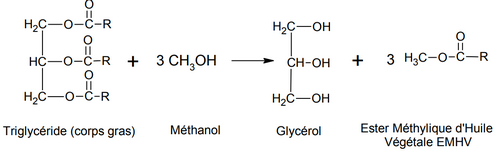
\includegraphics[scale = 0.85]{EMHV.png}
	\caption{Réaction de synthèse d'un EMHV à partir de méthanol et d'une huile végétale.}
	\end{center}
\end{figure}

	\subsubsection{Choix du protocole}

Le méthanol est un alcool primaire extrêmement toxique et CMR. Les principes de la chimie verte nous suggèrent d'éviter son utilisation. Les recherches actuelles s'intéressent aux EEHV, \textbf{esters éthyliques d'huiles végétales}, produites à partir de l'éthanol, bien moins nocif.

	\subsubsection{Protocole : Terminale S Hachette, p444}

Nous allons mettre en œuvre une réaction de transestérification par catalyse basique entre un \textbf{triglycéride} (le linoléate de glycéryle, présent dans l'huile de colza) et l'\textbf{éthanol}.

\begin{itemize}
	\item Montage à reflux (ballon, chauffe ballon, boy, réfrigérant verre, alimentation en eau.
	\item 120 mL d'huile de colza, 60 mL d'éthanol, 1.1 g d'hydroxyde de potassium (KOH).
	\item 150 mL d'eau salée saturée, solution de chlorure d'ammonium.
	\item Agitateur magnétique en verre.
	\item Synthèse en préparation.
	\item Plonger le mélange réactionnel après 50 minutes de chauffe dans 150 mL d'eau salée saturée, 			agiter et \textbf{laisser décanter toute la préparation}.
\end{itemize}

	\subsubsection{Exploitation en direct}
	\begin{itemize}
		\item \textbf{Définition de transestérification :} c'est une réaction qui transforme un ester 				(le triglycéride linoléate de glycéryle) en un autre ester (le linoléate d'éthyle).
		\item Le linoléate de glycéryle est formé par estérification à partir d'acide linoléique et de 				glycérol. De façon générale, les triglycérides sont formés avec du glycérol et des acides 				gras (longue chaine carbonée).
		\item \textcolor{blue}{Équation bilan (figure)}. Écrire les quantités. Le biodiesel et l'huile 				de colza sont miscibles. Si on veut éviter d'avoir à séparer le trilinoléate de glycéryle 				du linoléate d'éthyle, il faut consommer totalement le réactif, d'où l'excès d'éthanol.
			La réaction va produire du glycérol en déchet. Les ions hydroxyde jouent le rôle de 					\textbf{catalyseur}, ils sont régénérés en fin de réaction.
		\item \textcolor{blue}{Présenter le montage à reflux succintement :} on chauffe pour accélérer 				la réaction et pour mieux homogénéiser le mélange, choix d'un réfrigérant à colonne de 					verre car on fait chauffer de l'éthanol, très volatil ($T_{eb} =$ 78\degree C). L'éthanol 				va se recondenser dans le ballon grâce au réfrigérant. Boy en position intermédiaire.
		\item Il faut réduire au maximum la teneur en eau du mélange réactionnel, pour éviter les 					réactions secondaires de saponification des triglycérides.
	\end{itemize}

	\begin{figure}[h!]
		\begin{center}
			\begin{tabular}{cc}	
			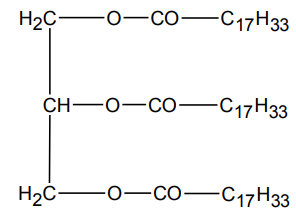
\includegraphics[scale = 0.45]{trilinoleate.png}& 
			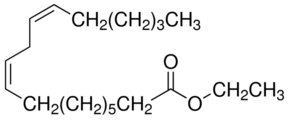
\includegraphics[scale = 0.5]{linoleate.png}\\
		\end{tabular}
		\end{center}
		\caption{Gauche : trilinoléate de glycéryle. Droite : linoléate de glycéryle (biodiesel)}
	\end{figure}

	\begin{figure}[h!]
		\begin{center}
		\begin{tabular}{c}
			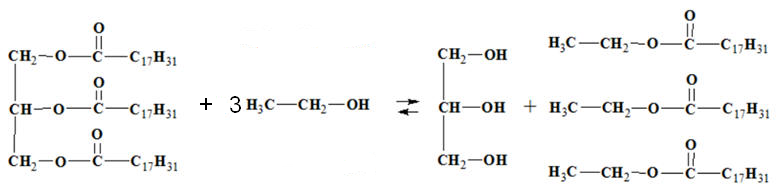
\includegraphics[scale = 0.55]{transester.png}\\
			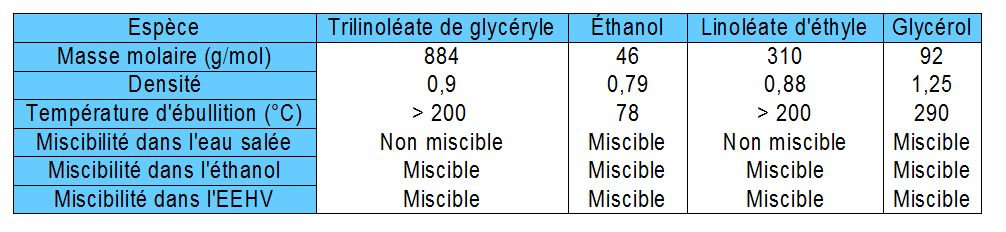
\includegraphics[scale = 0.50]{data_biodiesel.png}
		\end{tabular}
		\end{center}	
		\caption{Haut : réaction de transestérification entre le trilinoléate de glycéryle 
		et l'éthanol ; équation bilan de la synthèse du biodiesel. Bas : données de la réaction.}
	\end{figure}
	
	\begin{itemize}
		\item \textcolor{blue}{Expliquer l'intérêt de verser le mélange réactionnel dans de l'eau salée 		saturée}, c'est le \textbf{relargage} : l'éthanol et le glycérol sont miscibles dans l'eau 				salée, ce qui n'est pas le cas de l'huile de colza et du linoléate d'éthyle. On obtiendra donc 			deux phases liquides, qu'on pourra séparer avec une ampoule à décanter.
	\end{itemize}
	\begin{itemize}
		\item \textcolor{blue}{En direct :} récupérer le contenu du bécher (biodiesel plus déchets et			eau salée) et verser délicatement dans une ampoule à décanter, séparer les phases (la phase 			inférieure est la phase aqueuse à éliminer). On récupère la phase organique.
		\item Laver la phase organique au chlorure d'ammonium pour neutraliser les bases (hydroxyde).
		\item Sécher sur du sulfate de magnésium anhydre pour éliminer le reste de phase aqueuse avec 			filtration (sur papier plissé) pour récupérer le liquide.
		\item Rendement... ou pas, l'huile de colza n'est pas un produit pur, 
		donc difficile à évaluer.\\
	\end{itemize}

	\begin{itemize}
		\item \textbf{Caractérisation 1 :} de la phase aqueuse par test chimique. En présence d'une 			solution d'ions hydroxyde $\text{OH}^-$(aq) et d'ions cuivre (II) $\text{Cu}^{2+}$(aq), le 				glycérol donne un précipité indigo qui se différencie nettement de celui d'hydroxyde de 
		cuivre (II) $\text{Cu(OH)}_2$(s) obtenu sans glycérol. Dans 3 tubes à essais, réaliser les 				mélanges suivants :
		\begin{itemize}
			\item Tube 1 : 1 à 2 mL d'\textbf{eau distillée}, quelques gouttes de solution d'hydroxyde 					de sodium puis quelques gouttes de solution de sulfate de cuivre.
			\item Tube 2 : 1 à 2 mL de \textbf{phase aqueuse}, quelques gouttes de solution d'hydroxyde 				de sodium puis quelques gouttes de solution de sulfate de cuivre.
			\item Tube 3 : 1 à 2 mL d'\textbf{huile de colza}, quelques gouttes de solution d'hydroxyde 				de sodium puis quelques gouttes de solution de sulfate de cuivre.
		\end{itemize}
		Agiter et observer. Conclure.\\
		
		\item \textbf{Caractérisation 2 :} CCM, mélange pentane/diéthyléther à 20/1, échantillons
	\end{itemize}
	
\subsection{Valorisation du glycérol}

Le glycérol est un co-produit de la réaction de transestérification. Sa valorisation est déterminante pour l'équilibre économique de la filière de production du biodiesel et nécessaire selon les principes de la chimie verte.\\ 

Pour 100 kg de biodiesel (ou EMHV) produit, 10 kg de glycérol est récupéré. La valorisation du
glycérol est d’autant plus intéressante que son prix a diminué avec l'essor de la production du
biodiesel. Des recherches sont en cours pour exploiter le glycérol. Avec une production mondiale de 950 000 tonnes par an, le marché du glycérol a été en croissance depuis 2002 en raison du développement important de nouvelles applications dans les produits de soins personnels (agent hydratant, solvant et lubrifiant) et d'hygiène corporelle et dentaire (savons, shampoings, dentifrices, bains de bouche) ou dans l'industrie alimentaire (agent humectant, solvant d'arôme, émulsifiant, stabilisant et épaississant).

\subsection{Les agrocarburants sont-ils durables ?}

Le biodiesel est issu du colza, du tournesol, de l'olive etc... Il est mélangé à une faible quantité de gazole d'origine fossile (7\% en volume). Lorsqu'on veut évaluer le caractère durable d'un produit chimique, il convient d'examiner toute la chaîne de production : lors du broyage des graines (trituration), des déchets sont produits (tourteaux). Ils peuvent être utilisés dans l'élevage, pour nourrir les animaux. Nous avons vu que le glycérol pouvait être utilisé dans l'industrie chimique, dans de très nombreux secteurs d'activité.\\

L'utilisation des biodiesels pourrait permettre de réduire les émissions de gaz à effet de serre de près de 50\% par rapport aux combustibles fossiles. En tenant compte de la valorisation des co-produits (tourteaux, glycérol), l'efficacité énergétique d'un biodiesel est 2.2 : l'efficacité énergétique d'un biodiesel est le rapport entre l'énergie contenue dans le biodiesel et l'énergie non renouvelable dépensée de la culture à la livraison.\\

Cela dit, l'efficacité énergétique d'un biodiesel est limitée du fait du faible rendement à l'hectare des cultures telles que celles du colza :  si la France voulait entièrement substituer ses carburants fossiles par des biocarburants, l'ensemble de la surface agricole française devrait être mobilisée.\\ 

On peut énumérer de façon générale plusieurs avantages et inconvénients au développement des agrocarburants :

\subsubsection{Avantages :}
\begin{itemize}
	\item Ressources naturelles pouvant être produites en grandes quantités par l'agriculture.
	\item Production potentiellement moins polluante : à comparer à l'extraction pétrolière des sables 			bitumineux hautement polluants, marées noires, etc.
	\item Produits issus de la chimie durable eux-mêmes moins polluants que les produits pétroliers, 			contenant du soufre et autres polluants.
	\item Démarche à long terme, où il n'est plus à craindre la raréfaction du pétrole et des troubles 			qui en découleraient : hausse des prix, conflits, etc.
	\item Même si un biocarburant rejette du , celui-ci avait été fixé par la plante lors de sa 				croissance. La combustion des produits pétroliers rejette quant à elle du  qui était piégé 				dans le sous-sol, donc hors cycle du carbone : bilan carbone meilleur pour les biocarburants.
\end{itemize}
	
\subsubsection{Inconvénients :}
\begin{itemize}
	\item Les biocarburants sont accusés d'être une source de concurrence par rapport à la production 			alimentaire humaine, pouvant accentuer les difficultés des régions où l'accès à la nourriture 			est difficile.
	\item Quid de la déforestation qui serait engendrée pour produire de nouvelles terres cultivables ?
	\item L'agriculture n'est pas sans conséquence pour l'environnement : pesticides, épuisement des 			sols et des ressources, dont l'eau douce ...
	\item Même si le bilan carbone est meilleur qu'avec le pétrole, il persiste des rejets de 
	$\text{CO}_2$ avec les biocarburants.
	\item De même, l'énergie par unité de volume des biocarburants, dit "pouvoir calorifique
	inférieur" (ou PCI), est plus faible que celui des carburants fossiles. Cela signifie que l'on 			consomme plus de biocarburant que de carburants fossiles pour parcourir une même distance.\\
\end{itemize}

Cette transition pétrole/agro-ressources est également possible pour d'autres applications : matières plastiques, solvants, etc. Autrement dit, le pétrole serait remplaçable.

\section{Économie d'atomes et d'énergie}\label{sec:2}

Nous allons illustrer d'autres principes de la chimie verte, relatifs à une utilisation plus responsable, plus économe, de la matière et de l'énergie.

\subsection{Principe d'économie d'atomes}

Pour minimiser les quantités de déchets produits, la chimie verte propose de réduire le nombre de sous-produits lors d'une réaction. On mesure l'efficacité d'un procédé visant à économiser les atomes avec l'EA (l'économie d'atomes, appelée aussi Utilisation Atomique) :
\begin{equation}
	\boxed{EA = \frac{\sum_i a_i M_i\text{(produits)}}{\sum_i b_i M_i\text{(réactif)}}}
\end{equation}
où $a_i$ et $b_i$ désignent les nombres stoechiométriques figurant dans l'équation bilan et $M_i$ les masses molaires des composés chimiques. On ne prend en compte que les produits \textbf{recherchés} et l'\textbf{ensemble des réactifs nécessaires}. Si cette quantité tend vers 1, le procédé est efficace en terme d'économie d'atomes.

\subsection{Comparaison de trois protocoles}

On compare trois protocoles de synthèse de l'arôme de poire, l'acétate d'isoamyle (éthanoate d'isoamyle). La réaction part de l'alcool isoamylique (3-méthylbutan-1-ol), que l'on fait réagir avec :
\begin{itemize}
	\item de l'acide éthanoïque : réaction d'estérification classique, 
		équilibrée avec un rendement de 67\%;
	\item de l'anhydride éthanoïque (formé à partir de deux molécules d'acide éthanoïque en retirant 			une molécule d'eau) : réaction totale d'estérification;
	\item de chlorure d'éthanoyle (un composé de la famille des chlorures d'acyle, dérivés des acides 			carboxyliques).\\
\end{itemize}

On souhaite déterminer quel protocole s'inscrit le mieux dans le cadre d'une chimie durable. Les réactifs et produits obtenus sont de coûts et de dangerosités similaires. Nous allons donc nous fonder sur l'Utilisation Atomique de chaque procédé, en supposant que le seul produit d'intérêt est l'acétate d'isoamyle, pour trancher :
\begin{equation}
	UA_1 
	= \frac{M(\text{acétate})}{M(\text{alcool}) + M(\text{acide})} 
	= 0.878 \quad\text{soit}\quad 87.8\%,
\end{equation}
\begin{equation}
	UA_2 
	= \frac{M(\text{acétate})}{M(\text{alcool}) + M(\text{anhydride})} 
	= 0.684 \quad\text{soit}\quad 68.4\%,
\end{equation}
\begin{equation}
	UA_3 = \frac{M(\text{acétate})}{M(\text{alcool}) + M(\text{chlorure})} 
	= 0.781 \quad\text{soit}\quad 78.1\%.
\end{equation}

On se lance dans le premier protocole, pour lequel l'UA est la meilleure, bien que le rendement soi plus faible. Si on souhaitait privilégier le rendement, le protocole 2 serait le meilleur. Les anhydrides d'acide et les chlorures d'acyle réagissent vivement (la réaction est totale, exothermique et rapide), notamment avec l'eau. On préfère utiliser les anhydrides, qui sont moins réactifs que les chlorures d'acyle.

\subsection{Synthèse de l'éthanoate d'isoamyle}
(Le Maréchal, Tome 2, page 76 : voir note de bas de page, p 77 pour les quantités)

Un chauffage au cœur de la matière assurant un gain de temps considérable (les synthèses se font en quelques minutes !). Chauffer moins longtemps réduit le risque de favoriser des réactions parasites, impliquant une amélioration du rendement.\\

On va utiliser un four à micro-ondes pour chauffer le milieu réactionnel : les micro-ondes pénètrent en profondeur dans la matière et permettent de chauffer le milieu sans passer par le biais de la conduction thermique. L'énergie est directement déposée dans le mélange réactionnel et pas dans le récipient.

\begin{itemize}
	\item Faire une synthèse complète en préparation, une autre avec une seule irradiation en direct 		(ou alors ne pas faire le biodiesel en manip).
	\item Acide éthanoïque en excès (on l'élimine facile par lavage à l'eau, contrairement à l'alcool 		et à l'ester qui ne sont pas simples à séparer).
	\item L'évaporation de l'eau par le micro-ondes déplace l'équilibre, d'où une amélioration du 			rendement.\\
	
	\item \textbf{Caractérisation :} indice de réfraction (linalol $n =$ 1.4623, produit $n =$ 1.4544) 		ou CCM cyclohexane/diéthyléther 3/1, révélation à l'acide phosphomolybdique.\\
\end{itemize}

Les micro-ondes possèdent la particularité d'interagir avec les molécules présentant un moment dipolaire permanent non nul, créant ainsi par basculements rapides des molécules résultant d'interactions avec le champ électrique alternatif, un échauffement local par agitation moléculaire. Le mode de chauffage fait que l'on peut rapidement faire monter un solvant en ébullition, ce qui peut représenter un danger. 

\section{Solvants et valorisation du $\text{CO}_2$}

De nombreux solvants organiques sont dangereux pour l'environnement et pour la santé. On citera par exemple
\begin{itemize}
	\item le benzène, très volatif et inflammable, cancérigène et mutagène utilisé comme précurseur 		dans de nombreux procédés de chimie organique, comme additif dans l'essence et autrefois comme 			solvant dans les colles, les vernis, les peintures;
	\item le toluène, nocif et reprotoxique;
	\item le dichlorométhane, cancérigène.
\end{itemize}
Ils sont de plus issus de l'industrie pétrochimique.\\

On cherche à remplacer ces solvants par d'autres moins nocifs, ou issus de l'agriculture : par exemple le glycérol ou les esters d'acides gras dont nous avons déjà discuté. D'autres solutions sont possibles, comme l'eau ou le dioxyde de carbone supercritiques.

\newpage
\subsection{Oxydation hydrothermale de déchets}

La plupart des déchets organiques liquides issus de l'industrie sont détruits par incinération. Cette technique est coûteuse en énergie et néfaste pour l'environnement. Dans certains cas, il est possible de la remplacer par la \textbf{conversion hydrothermale}.\\

Au-delà d'une température et d'une pression bien précises, appelées \textbf{température et pression critiques}, l'eau entre dans un état dit \textbf{supercritique} ni entièrement liquide ni entièrement gazeux, caractérisé par des fluctuations de densité importantes. Un tel fluide possède une bonne capacité de solvatation et facilite le transport de matière (faible viscosité, diffusion moléculaire élevée). L'eau supercritique peut donc servir de solvant.
	
\begin{figure}[h!]
	\begin{center}
	\begin{tabular}{cc}
		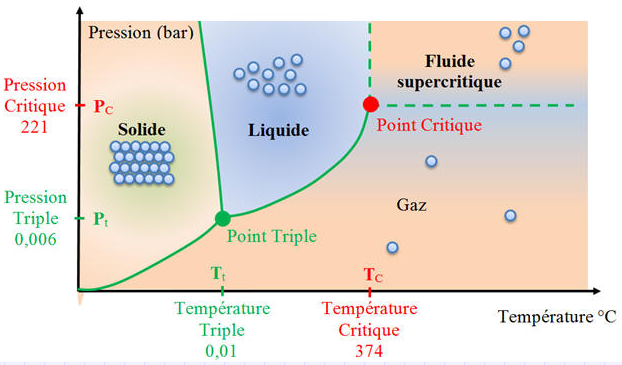
\includegraphics[scale = 0.4]{supercrit.png}&
		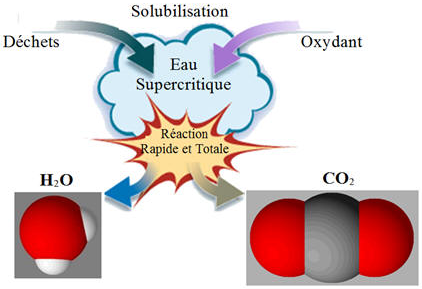
\includegraphics[scale = 0.5]{hydrothermale.png}\\
	\end{tabular}
	\end{center}	
	\caption{Gauche : diagramme de phase de l'eau. Droite : principe de l'oxydation hydrothermale.}
\end{figure}
	
Le traitement des déchets organiques toxiques peut être réalisé avec de l'eau supercritique : le dioxygène et les composés organiques sont solubilisés et les réactions d'oxydation favorisées. Elles deviennent quasi totales et rapide, le contact entre les réactifs étant meilleur.

Les produits sont de l'eau et du dioxyde de carbone. L'eau est ramenée à l'état liquide par refroidissement et les éléments métalliques, les minéraux et les hétéroatomes se retrouvent dans la phase aqueuse sous forme dissoute (ions) ou sous forme de précipités. On les traite ensuite par des procédés classiques (décantation, filtration etc...). Ce procédé se fait à des températures relativement faibles (de l'ordre de 100\degree C) et ne produit pas d'oxydes d'azote ou de soufre, gaz impliqués dans les mécanismes de pollution atmosphérique.

\subsection{Valorisation du dioxyde de carbone}

Le point critique du dioxyde de carbone est atteint pour $T = 304.25$ K et $p = 72.9$ atm. Il peut être utilisé dans son état supercritique comme solvant d'extraction. L'extraction au dioxyde de carbone supercritique se substitue à une extraction par solvant liquide classique. 

Pour l'exemple, l'industrie du café décaféiné des années 1970 utilisait du chloroforme pour extraire la
caféine. Mais les consommateurs commencèrent à présenter des affections du type cirrhose du foie. L'utilisation du $\text{CO}_2$ SC a permis d'obtenir un café sans trace de solvant.

\subsection{Liquides ioniques}

Les liquides ioniques sont des sels possédant une température de fusion inférieure à 100\degree C et sont, pour beaucoup, à l'état liquide autour de la température ambiante. Ils forment en fait une nouvelle classe de solvants à part entière qui offrent d'intéressantes opportunités comme milieu réactionnel pour une chimie plus propre. Ces sels sont constitués de cations organiques complexés avec des anions inorganiques ou organiques. Leurs avantages sont multiples :
\begin{itemize}
	\item pas volatiles à température ambiante (pas de diffusion dans l'atmosphère de 							produits toxiques ou inflammables)
	\item stables à haute température,
	\item rarement inflammables.
\end{itemize}
Les liquides ioniques constituent globalement de bons solvants pour de nombreux composés organiques et inorganiques.

\section*{Conclusion}

Durant cette leçon nous avons illustré plusieurs concepts de la chimie verte dans le contexte de la chimie organique (synthèses à partir de ressources issues de l'agriculture, économie d'atomes et d'énergie, traitement de déchets et remplacement de solvants toxiques par des solvants moins dangereux.\\

La chimie peut également apporter des solutions en matière de production d'énergie propre, en utilisant par exemple les réactions d'oxydoréduction. Une \textbf{pile à combustible} est un générateur dans lequel la fabrication de l'électricité se fait grâce à l'oxydation sur une électrode d'un combustible réducteur (par exemple dihydrogène) couplée à la réduction sur l'autre électrode d'un oxydant, tel que le dioxygène de l'air. La réaction d'oxydation de l'hydrogène est accélérée par un catalyseur qui est généralement du platine. Si d'autres combinaisons sont possibles, la pile la plus couramment étudiée et utilisée est la pile dihydrogène-dioxygène (ceci s'expliquant notamment par l'abondance des ressources en hydrogène sur Terre et la facilité de production du dihydrogène). Le seul produit de la réaction est l'eau, d'où l'intérêt de ce type de générateur.

\newpage
\section*{Annexes}

\subsection{Générations de bio-carburants}

Les biocarburants dits de première génération, qui sont actuellement sur le marché sont issus des réserves énergétiques (graisse, amidon, sucre) des plantes ou des animaux et, de façon encore marginale de la collecte d'huiles usagées. Ils sont utilisés en mélange avec les hydrocarbures dans des proportions variant de quelque \% jusqu'à 85\%. En France, ils sont distribués pour la circulation automobile sous deux formes, le biodiesel en addition au gazole, le bioéthanol en addition à l'essence. \\

Le biodiesel est fabriqué en France essentiellement à partir d'huile extraite du colza et du tournesol
qui poussent sur place, du soja et du palmier pour la part importée. L'huile végétale brute n'est pas
utilisée telle quelle dans les moteurs mais sous forme d'un produit dérivé, dit ester méthylique d'huile végétale ou EMHV. Il est incorporé au gazole avec un taux, le plus souvent, de 7\% en volume. La production de biodiesel est automatiquement associée à celle de tourteaux de colza ou de tournesol,
composante de l'alimentation du bétail.\\

Le bioéthanol est, quant à lui, un alcool produit soit par la fermentation du sucre issu de plantes
(betteraves, cannes à sucre) soit par hydrolyse de l'amidon issu de céréales (blé, maïs). Il peut être
mélangé directement à l'essence avec des pourcentages allant de 5 à 85 \% en volume.
L'usage de l'éthanol à très forte concentration (par exemple 85 \% dans l'E85) nécessite une
adaptation spécifique du véhicule. C'est généralement à des faibles teneurs qu'il est utilisé (5 à 10\%
par exemple dans l'E10).\\

La production d'éthanol génère des coproduits (pulpe de betterave, drèches de blé ou de maïs) qui sont une base de l'alimentation animale, compte tenu de leur haute teneur en protéines. Il en est de même pour la filière diesel qui produit du glycérol, molécule valorisée dans des voies de synthèse.\\

\textbf{Seconde génération :} l'intérêt des biocarburants 2ème génération est d'utiliser la plante entière en valorisant les différents constituants du végétal. Les choix portent sur l'utilisation de plantes limitant les concurrences avec d'autres usages traditionnels (alimentation humaine ou animale, industrie du bois ...) mais aussi présentant des avantages agronomiques et environnementaux (limitation des consommations d'eau, d'engrais, de produits phytosanitaires ...).\\

\textbf{Troisième génération :} certaines espèces de microalgues peuvent fixer le $\text{CO}_2$ par le mécanisme de la photosynthèse et accumuler des quantités importantes de lipides (50 à 80\% en masse sèche) et constituent ainsi une source de biodiesel. Parallèlement, leur culture n'entre pas en compétition avec les terres agricoles. Autre avantage, la croissance des algues lipidiques nécessitant d'importantes quantités de $\text{CO}_2$, on peut envisager de recycler ainsi le $\text{CO}_2$ émis par des usines ou des centrales thermiques. De plus, la biomasse algale fournit des produits annexes à haute valeur ajoutée comme les protéines, les vitamines ou les oligo-éléments qui peuvent être valorisés (agroalimentaire, cosmétique, pharmacie, etc.). De nombreux verrous limitent actuellement la viabilité économique et environnementale de la filière de production de carburants à partir de microalgues.


\end{document}